% !TEX root = jbsilvaThesis.tex

%%%%%%%%%%

\pagebreak

\chapter{\label{chp:intro_quakes}Earthquake Fault Systems in the Real World}

\section{Introduction to Earthquake Fault Systems and Hydraulic Fracturing}

Empirically it has been determined that earthquake fault systems collectively display certain common properties including Gutenberg-Richter scaling for the frequency of seismic events. This type of scaling is more generally known as power law scaling. Any valid model for earthquake fault systems must agree with Gutenberg-Richter scaling obtained from geophysical data. My focus is  on one such model for an earthquake fault system known as the \ofc\ model~\cite{ofc92}. This model will be described in greater detail in Section~\ref{sect:ofc}.

Technological improvements in natural gas extraction has led to an increase in the amount of natural gas wells in the United States. The most well known of these gas extraction methods in the United States is known as hydraulic fracturing. Hydraulic fracturing is a process of extracting gas from shale rock by creating micro fractures in the rock by injecting a fluid at a high pressure into the well. These micro fractures release natural gas from the shale rock which can then be collected. 

The popularity of this extraction technique has increased in Oklahoma from a single digit amount of well sites in 2005 to nearly a thousand in 2015 as estimated from well servicing logs. In recent years the increase in  seismic activity has been of interest in areas such as Oklahoma where a large amount of hydraulic fracturing activity is occurring. Naturally any changes in the local physical system caused by this process are of interest. The development of models for earthquake fault systems undergoing hydraulic fracturing would aid in understanding how  hydraulic fracturing  could change the frequency of events as well determining how unique any possible changes are to the individual fault systems.

A significant part of my research  will focus on modeling an earthquake fault system with an invasion percolation process occurring within the system as a model of hydraulic fracturing. It will be shown that such models create a deficit in the number of small events compared to the event frequency in the standard \ofc\ model. 
% It will be shown that ergodicity is not preserved, which justifies the idea that the evolution of the earthquake fault system is not comparable across different well sites where hydraulic fracturing occurs.


\section{The Properties of Earthquake Fault Systems}

The empirical study of earthquakes has led to the discovery  of empirical laws for the behavior of earthquakes including Gutenberg-Richter scaling~\cite{gr56}, Bath's law~\cite{bath65}, and Omori's law~\cite{omori94}. These empirical laws has been the subject of interest by researchers in seismology, geophysics and physics. Gutenberg-Richter scaling relates the frequency of seismic events of a given size and is summarized in Eqn.~\eqref{eq:gutrichscaling} for a scaling exponent $\beta$ which relates the number $N$ of seismic events to the seismic moment $M$. Seismic moment is a combination of the area of fault slip, the average amount of slip, and the force to overcome the friction.
%%
\begin{equation}
 \label{eq:gutrichscaling}
	N \propto M^{-\beta}.
\end{equation}

\begin{equation}
 \label{eq:omori}
	n(t) = \frac{k}{(t+C)^1}
\end{equation} %%
% 
Omori's law has not received the focus that  Gutenberg-Richter scaling has. In this thesis work is done focusing on Omori's law~\cite{omori94} which relates the number of aftershocks after a given time from the main seismic event as given by Eqn.~\eqref{eq:omori}. An important step in this work will be modeling the effects of asperities in an earthquake fault system by extending the \ofc\ model~\cite{ofc92} to include the effects of asperities. 

\section{Block-spring Models for an Earthquake Fault System}
\label{sect:blocksprings}
One of the early models of an earthquake fault system is the \bk\ model~\cite{brkp67}. In this model the system is represented by a system of blocks interconnected by linear springs. The blocks are also connected to a ``loader" plate that rests on  rough surface with Mohr-Coulomb friction. The spring constant of the springs between the loader plate and blocks is given by $K_L$ and the intrablock spring constant is $K_c$. The block displacement, which is also known as the \emph{slip deficit}, is denoted by $\phi$. The stress on a block is defined by %%
%%
\begin{equation}
 \label{eq:stress}
 \sigma_i = -K_L \phi_i + K_c \sum (\phi_j-\phi_i) . 
\end{equation}  %%
%%
As the loader plate moves the stress on all the blocks is increased and the possibility of a block slipping increases. A block slips once the stress on the block exceeds a predefined failure threshold. Once the block slips, its displacement is adjusted as dictated by Newton's equations of motions resulting in the displacement adjustment given by Equation~\eqref{eq:displacement}.
%% solved from newtons equation equation of motion.
\begin{equation}
 \label{eq:displacement}
  \phi_f = \phi_i + \frac{\sigma_i - \sigma_R}{K_L +  qK_c} 
\end{equation} %%
%%
This change in displacement of the blocks decreases the stress on the block that has slipped, but generates stress on the blocks connected to the slipping block. This stress transfer can initiate a failure in these connected blocks, possibly initiating an avalanche of  ``failed'' blocks. The minimum size of an avalanched is one composed of the initial failing block. Additionally a condition will be imposed in which a loader plate moves slowly enough that only a single site fails that is referred to as the \textit{zero velocity limit} in the literature. 

% clarify difference between rjb and bk model
The \rjb\ model proposes simplifications to the \bk\ model in which a block's motion occurs before the connected blocks can move. These simplifications lead to a cellular automaton model with two primary variables given by the stress and displacement. The dynamics of the \rjb\ model with the zero velocity limit are summarized in the following:    %%
%% 
\begin{itemize}
	\item System of blocks with displacements $\phi$.
	\item Stress on block $i$ is computed using  $ \sigma_i = -K_L \phi_i + K_c \sum_j (\phi_j-\phi_i) $.		
	\item The loader plate is moved until a single site fails (\emph{zero velocity limit}). 
	
	\item The displacement of the failed block  is reassigned:    
				$ \phi_f = \phi_i + \frac{\sigma_i - \sigma_R}{K_L +  qK_c}  $.
\end{itemize}
%%
The presence of springs allows for a simple definition of the total energy by summing the energy of springs connecting the blocks to  other blocks as well as the energy of the springs connecting the blocks to the loader plate.  %%
%%
\begin{equation}
 	\label{eq:rjbenergy}
	E_{\rm RJB} = E_{\rm plate,block}+E_{\rm block,block} =\sum \frac{1}{2} [ K_l \phi_i^2 + \sum_{j\in \rm range\, R } K_c (\phi_i-\phi_j)^2 ]
\end{equation}  %%
%%
				 
\section{The \ofc\ Model}%%
\label{sect:ofc}
%%
\begin{figure}
% move to closer to event size histogram
  \centering
	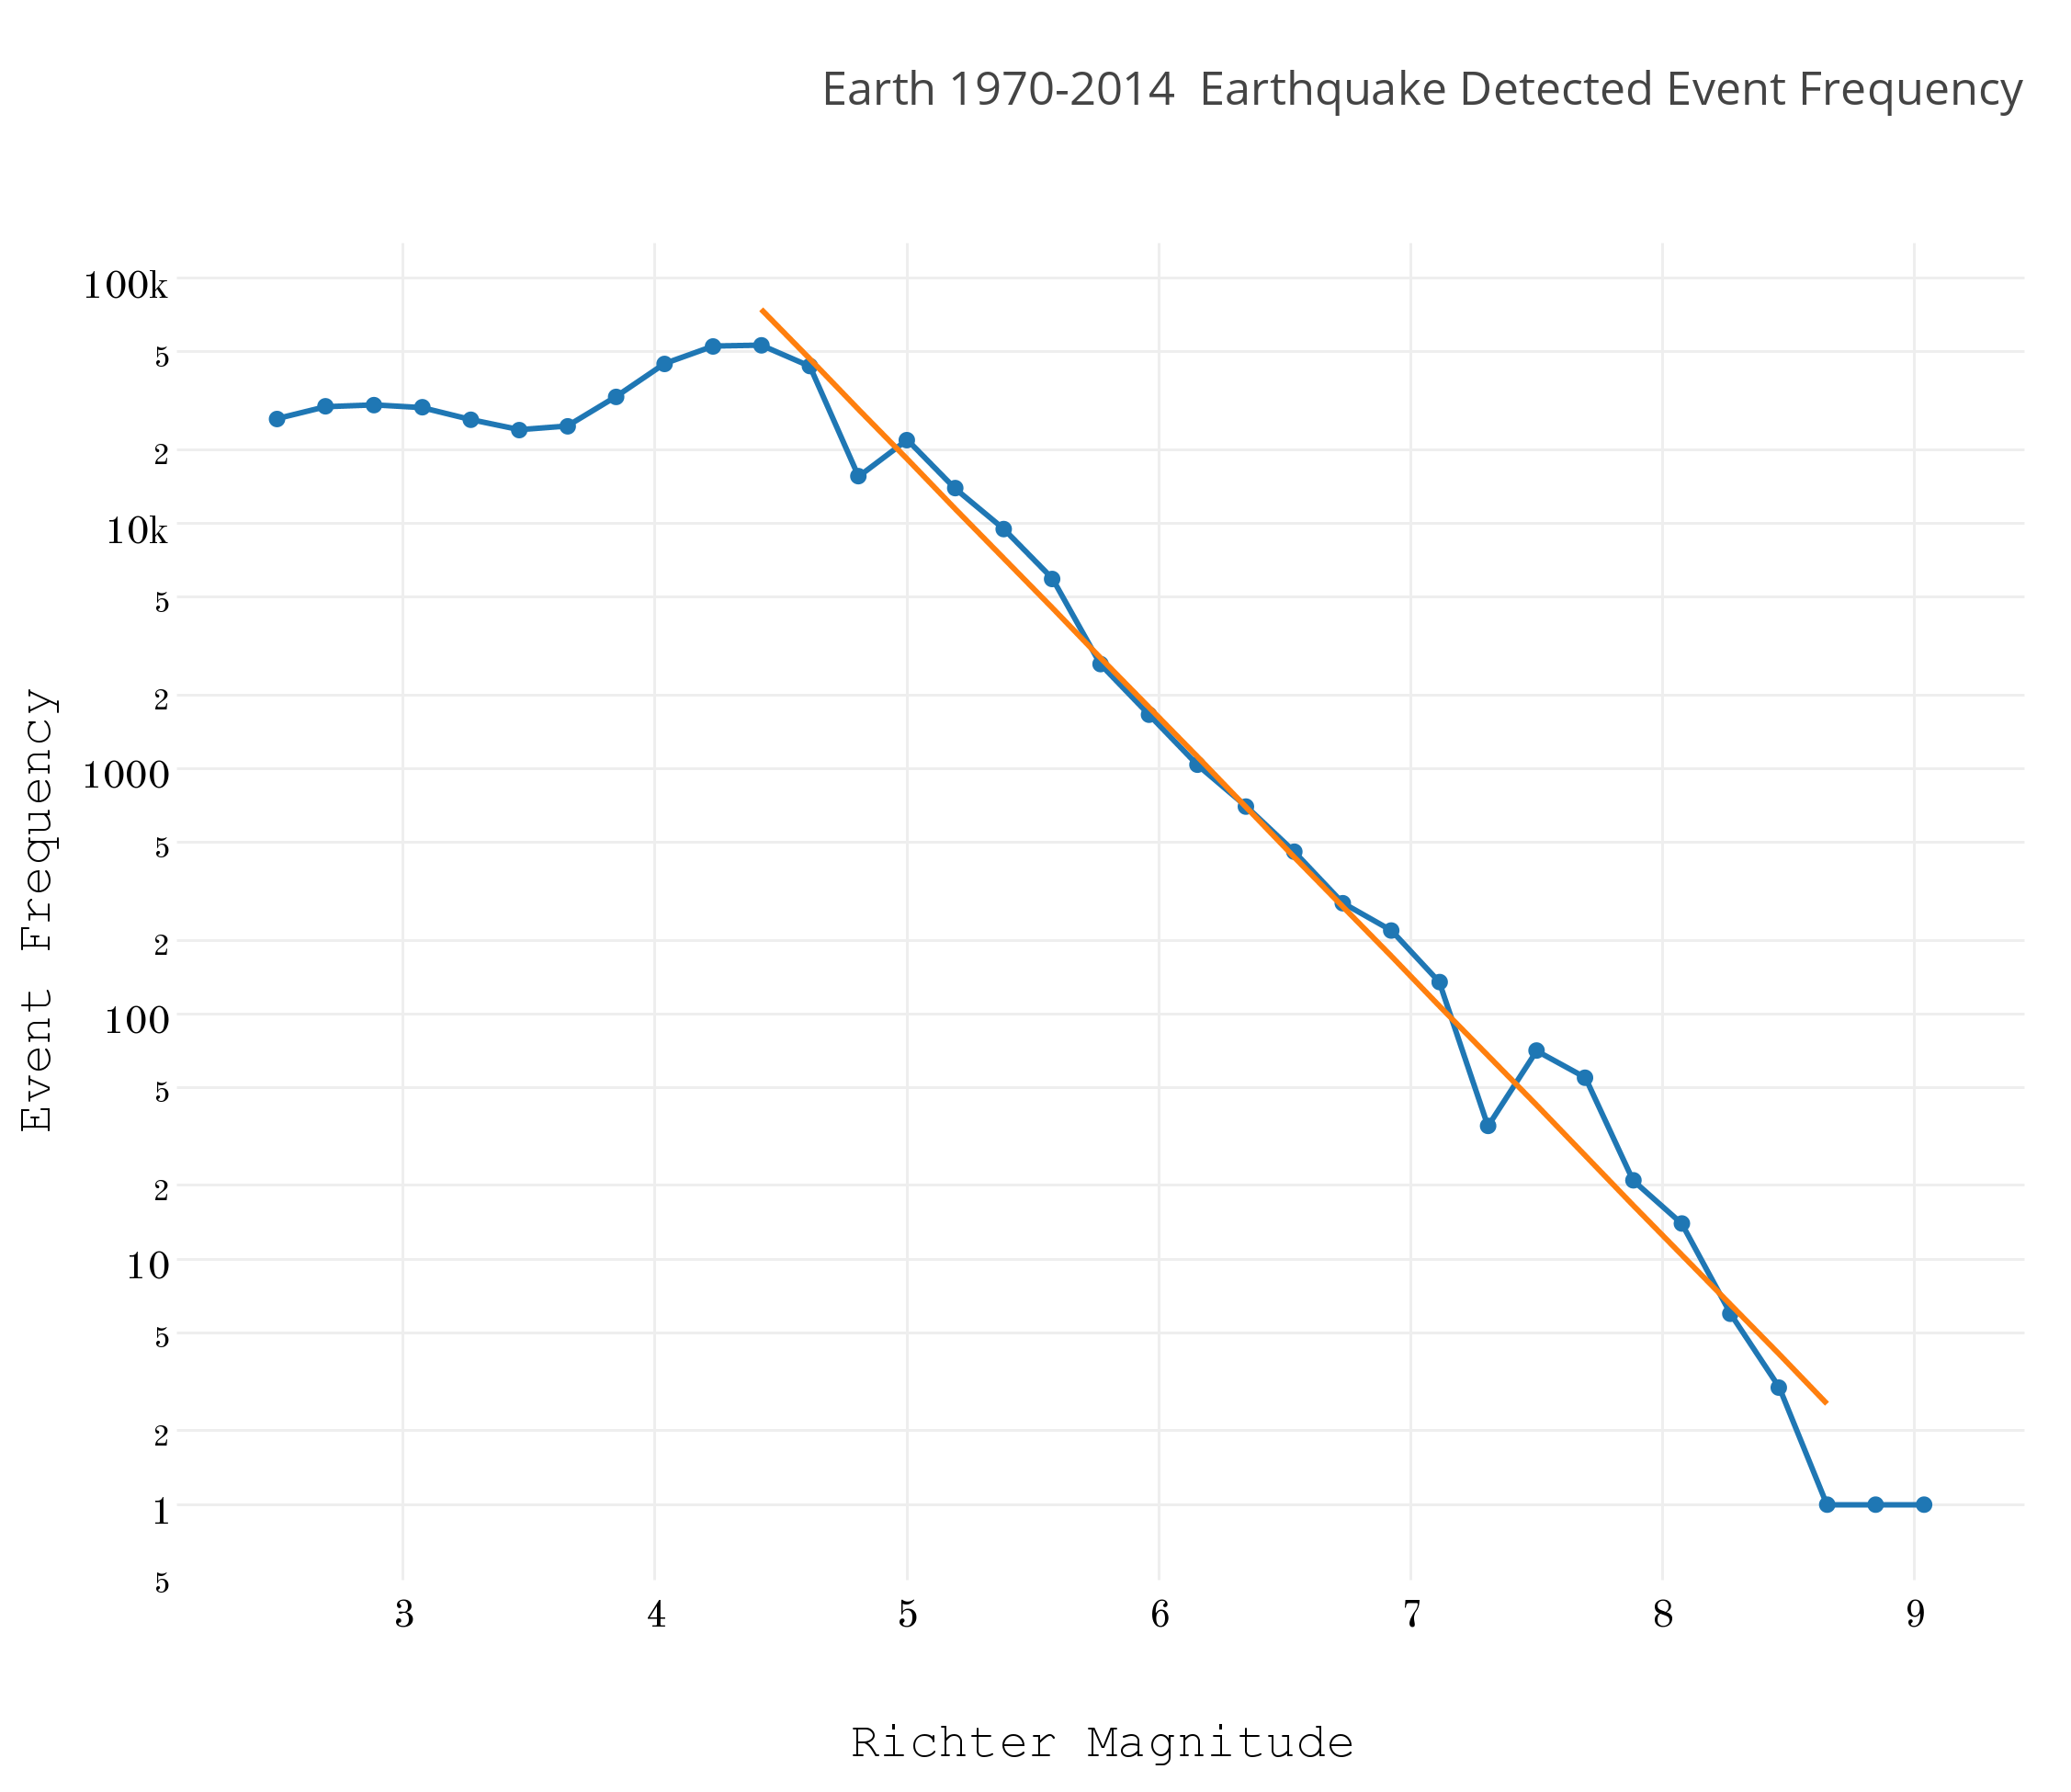
\includegraphics[width=0.70\textwidth]{{Images/earth_1970-2014__earthquake_detected_event_frequency}.png}
  \captionof{figure}{Event frequency distribution for all USGS API earthquake events.}
  \label{fig:earthevents}
\end{figure}%%
\begin{figure}
  \centering
	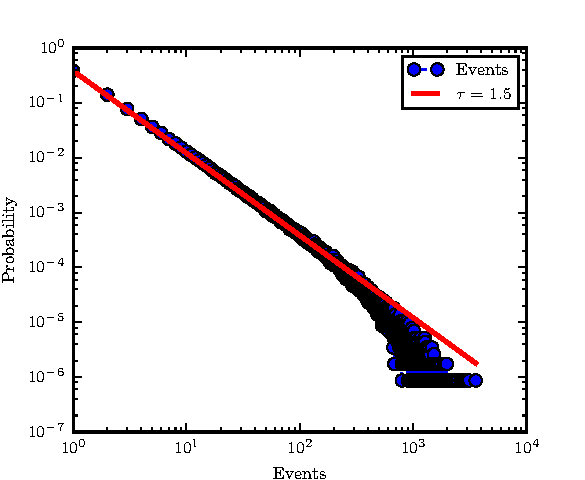
\includegraphics[width=0.7\textwidth]{{Figures/ofc/SumSqHistEvt8L120-alph1-500-noise-220000}.pdf}
  \captionof{figure}{\ofc\ event size histogram for $\alpha=0.05$, $L=120$, and $R=8$. }
  \label{fig:ofcevts}
\end{figure}%%
%% ofc and rjb both cellular autamaton models and both does not have inertia
In 1992 Olami, Feder, and Christensen proposed a cellular automaton model to study self-organized criticality~\cite{ofc92}. This model was discovered independently from the block-spring \rjb\ model for earthquake fault systems. The \ofc\ model is  composed of a lattice of sites with a stress variable $\sigma$ analogous to the displacement between blocks in a block spring system as well as the displacement between blocks and a loader plate which introduces stress in the system. Once the stress on a given site exceeds the  failure threshold, the site slips and returns to a lower stochastically assigned residual stress value. The latter has a mean value and a stochastic noise term denoted by $\eta$. The difference of the the stress at the time of failure and the residual stress is partially dissipated while the rest of the excess stress is distributed to the neighbors of the failed site. This process of redistributing stress is repeated until there are no more failed sites in the lattice. The size of an event is the number of sites that fail. 
\begin{itemize}
	\item  \textbf{\ofc\ Model Dynamics} 
\begin{itemize}
	\item Lattice of sites with stress $\sigma_j$ at site $j$.
	\item System is loaded until a single site fails (\emph{the zero velocity limit}). 
	\item Stress on failing site returns to residual level plus a random noise. 
	\item Excess stress on failed site given by the following equation is dissipated to sites using \lr\ stress transfer.
	\begin{equation}
	\sigma_{\rm diss} = (1-\alpha) [\sigma_i- \sigma_f] = (1-\alpha) \Delta \sigma
	\end{equation}		
\end{itemize}
\end{itemize}%%
%%
\subsection{What properties are universal?}
% move to intro
A cornerstone of any physical model is its agreement with empirical results. This leads to a set of properties that any possible earthquake model must satisfy to be  useful. As discussed, the most famous property  of earthquakes is given by Gutenberg-Richter scaling~\cite{gr56} which relates the number $N$ of events of Richter magnitude $M$ or greater. %%
%%
\begin{equation}
 \label{eqn:grscaling}
	N = 10^{a-bM}
\end{equation} %%
%%
The scaling in Eqn.~\eqref{eqn:grscaling} can be transformed to a power law if the magnitude is replaced by the seismic moment. It is believed that Gutenberg-Richter scaling is associated with the earthquake fault system being near criticality. In a system near criticality as discussed in Chapter~\ref{chp:nuc_details} there are  clusters with a critical exponent $\tau$ describing the cluster size scaling. As discussed by Serino et al.~\cite{serinoth} the critical exponent $\tau$ is related to the $\beta$ exponent in Equation~\eqref{eq:gutrichscaling}.


Due to the ambiguity in the distinction of a main shock and an after shock Gutenberg-Richter scaling also applies to earthquake aftershocks. Aftershocks also have empirically derived behavior including Omori's law~\cite{omori94} and Bath's law~\cite{bath65}. Bath's law concerns the observation that there is a constant difference in the Richter magnitude between a main shock and its largest aftershock. Sornette and collaborators have argued that Bath's law is a consequence of other aftershock properties and Gutenberg-Richter scaling~\cite{sornette03}. Omori's law relates the time scale to the rate of large aftershocks as given in Eqn.~\eqref{eq:omori}. %%
%%
\begin{equation}
 \label{eq:omori}
	n(t) = \frac{k}{(t+C)^1}
\end{equation} %%
%%
The exponent of $1$ in Eq.~\eqref{eq:omori} was shown to actually be a range of values by  Utsu et al.~\cite{utsu95}. Omori's law is of particular interest because  my work on asperities is motivated by explaining the possible cause of Omori's law. In particular, the interactions of asperities with each other will be particularly valuable in understanding Omori's law.


\subsection{ Theory for statistical analysis of earthquake fault systems in \lr\ stress transfer }

In this section the results of Klein et al.~\cite{kleinferg13} will be followed to elucidate the relation between spinodal nucleation and earthquake fault system behavior in the limit of \lr\ stress transfer. 
% more obvious -> identification in the long range ofc 

In the work of Klein et al.\ the \rjb\ model is spatially coarse grained to a block the size of the \lr\ stress range as well as coarse grained in time. This coarse grained system can be described by a $\phi^4$ theory. A spinodal is then associated with a large value of the total coupling constant $K=K_L+K_c$. There is an arrested   spinodal nucleation between a stable high stress phase and a metastable low stress phase. The high stress phase is inhibited by  metastable phase decay in the form of an earthquake event which releases stress resulting in a return to low stress. The number of failed sites in an event in the \rjb\ model  gives a measure of the size of an event.

In the work of Serino et al.~\cite{serino11}  scaling  is further extended to a system with damage in the form of ``dead sites" that simply dissipate any stress distributed to the site.

\subsection{Connecting earthquake fault models}

Earthquake fault modeling is possible using many approaches that may appear distinct but can possibly be different reinterpretations of the same models. By focusing solely on the dynamics of the stress in the \rjb\ model one can form a concrete analogy to the \ofc\ model. This can be further quantified by calculating the dissipation in stress resulting from Eqn.~\eqref{eq:displacement}. The resulting relation to the dissipation $\alpha$ is given by the following equation for a given loader plate to the block spring constant $K_L$, block to block spring constant $K_c$, and the number of blocks $q$ within the \lr\ stress transfer range.  %%
%%
\begin{equation}
 \label{eq:ofcrjbalpha}
	\alpha = \frac{K_L}{K_L + qK_c}
\end{equation}%%
%%
Equation~\eqref{eq:ofcrjbalpha} allows for the mapping of the spring constants to  a single dissipation value. This mapping is incomplete without  variables such as the energy of the \ofc\ that may possibly connect this driven dissipative system to equilibrium statistical physics methods. Due to the linear nature of the stress to the displacement in the \rjb\ model one may propose an approximation to the energy in the \ofc\ model given by Eqn.~\eqref{eq:ofcenergy}.   %%
%%
\begin{equation}
 \label{eq:ofcenergy}
	E_{\rm ofc} \propto \sum_i \sigma_i^2
\end{equation}%%


In the \ofc\ model the strength of the residual noise applied to the system is the analogous temperature variable. Given a system in thermal equilibrium the probability of the energy will follow a Maxwell-Boltzmann distribution given by Eqn.~\eqref{eq:maxwellboltz}, where $\rho(E)$ is the density of states which is independent of the temperature, and $\beta=\frac{1}{k_B T}$.
%%
\begin{equation}
 \label{eq:maxwellboltz}
	P(E,\beta) = \rho(E) e^{ -\beta E }
\end{equation}%%
%%
Given two systems in thermal equilibrium following Maxwell-Boltzmann distributions ($\beta_1 < \beta_2$) at varying temperatures Eqn.~\eqref{eq:maxwellboltzrat} is obtained. %%
%%
\begin{equation}
	\label{eq:maxwellboltzrat}
	\frac{P(E,\beta_1)}{P(E,\beta_2)} \propto e^{ -(\beta_1-\beta_2) E }
\end{equation} %%
%%
Lastly the logarithm of Eqn.~\eqref{eq:maxwellboltzrat} results in Eqn.~\eqref{eq:maxwellboltzratlog}. %%
%%
\begin{equation}
	\label{eq:maxwellboltzratlog}
	\log ({\frac{P(E,\beta_1)}{P(E,\beta_2)}}) =  -\Delta \beta E + b 
\end{equation}%%

\begin{figure}[!h]
    \centering
      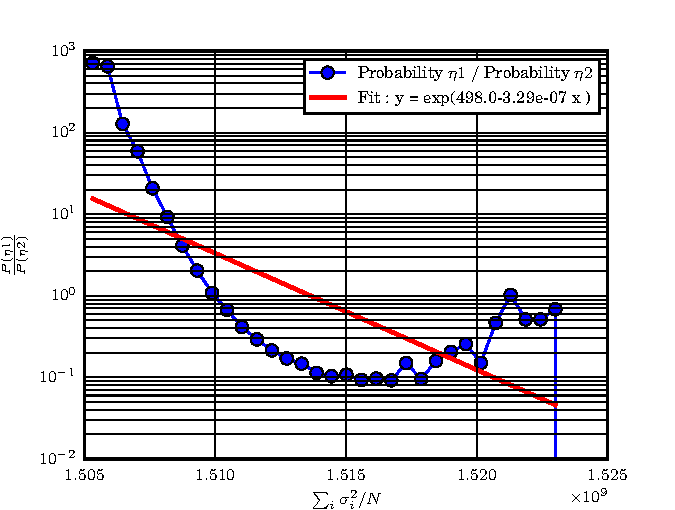
\includegraphics[scale=1.1]{{Figures/sumsq/sumSqHistLogRNNL250-alph1-0.01}.pdf}
    \caption{Ratio of probabilities of the total energy   for the nearest-neighbor \ofc\ model for $\alpha=0.01$ and $L=250$. } 
  \label{fig:nnratiosumsq}
\end{figure}%%

Equation~\eqref{eq:maxwellboltzratlog} will be used to determine if a given energy definition is plausible for the  \ofc\ model. The equivalent dynamics of an \ofc\ model and a model with properly chosen spring constants in the 
\rjb\ model will be used as a verification  of this work. The nearest-neighbor stress transfer \rjb\ model has been previously understood to not display equilibrium behavior in its well defined energy~\cite{sornette97}. An equivalent \ofc\ with the parameters $\alpha=0.01$, $L=250$, and $R=1$ was chosen to measure the proposed energy definition at two distinct residual noise values $\eta=5.0$ and $\eta=5.15$. Figure~\ref{fig:nnratiosumsq} displays the resulting nonlinear behavior of the proposed energy as expected from the analogous 
\rjb\ results.    

%%
\begin{figure}[!h]
    \centering
      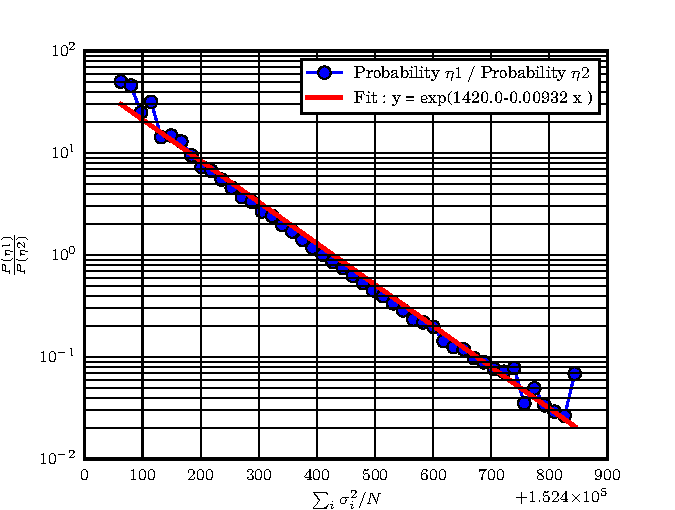
\includegraphics[scale=1.2]{{Figures/sumsq/sumSqHistLogR30L512-alph1-0.01}.pdf}
    \caption{ Total energy probability ratio for an \ofc\ model with $\alpha=0.01$, $L=512$, and $R=30$. A fit to the Boltzmann distribution is observed. } 
  \label{fig:longrangeratiosumsq}
\end{figure} %%
%%			
This equation will be used to determine if a given energy definition is plausible for the given \ofc\ system. The equivalent dynamics of an \ofc\ model and a model with properly chosen spring constants in the \rjb\ model will be used as a verification of this work. A nearest-neighbor stress transfer \rjb\ model has been previously understood to not display equilibrium behavior in its well defined energy. An equivalent \ofc\ with the parameters $\alpha=0.01$, $L=250$, and $R=1$ was chosen to measure the proposed energy definition at two distinct temperature analogs residual noise values $\eta=5.0$ and $\eta=5.15$. Figure~\ref{fig:nnratiosumsq} displays the resulting non linear behavior of the proposed energy as expected from the analogous 
\rjb\ results.    

It is only at larger stress transfer ranges that the 
\rjb\ energy displays equilibrium behavior, implying that an  equivalent \lr\ \ofc\ models should also display such equilibrium behavior. In Fig.~\ref{fig:longrangeratiosumsq} a \lr\ stress transfer \ofc\ model is observed with  $\alpha=0.01$, $L=512$, and  $R=30$. In this system one observes the expected linear behavior for the proposed \ofc\ energy. To confirm the analogous nature of the energy a \lr\   \ofc\ model  with $R=30$ was chosen along with the equivalent 
\rjb\ system. From Eqn.~\eqref{eq:maxwellboltzratlog} the slope of the energy term should be equivalent for the equivalent  systems.  

Figures~\ref{fig:ofcsumsq} and~\ref{fig:rjbsumsq} confirm this equivalence for equivalent systems sharing the parameters $\alpha=0.0476$, $L=144$, and $R=6$. The measured slopes of $648$ and $653$ as well as $y$-intercepts are within bootstrapped errors. %%
%%
\begin{figure}
\centering
\makebox[\textwidth][c]{
\begin{minipage}{.5\textwidth}
  \centering
	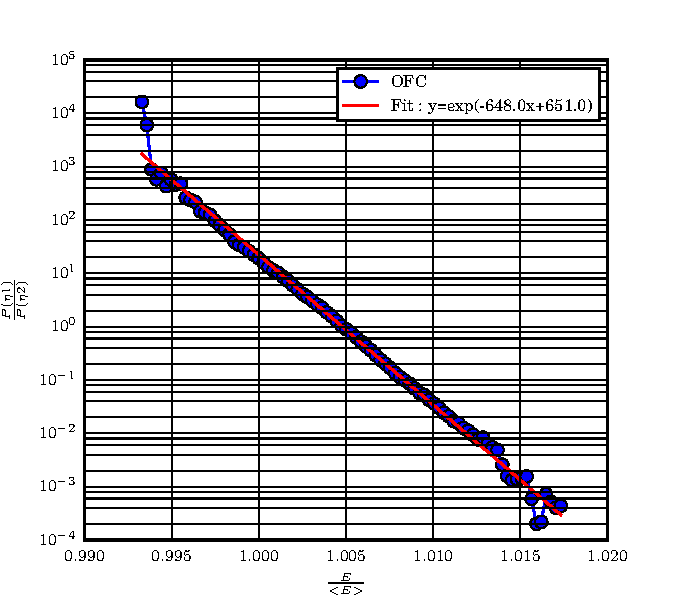
\includegraphics[width=1.0\textwidth]{{Figures/sumsq/OFCSumSqHistLogR6L144-alph1-476}.pdf}
  \captionof{figure}{Total energy probability ratio for \ofc. }
  \label{fig:ofcsumsq}
\end{minipage}%
\begin{minipage}{.5\textwidth}
  \centering
	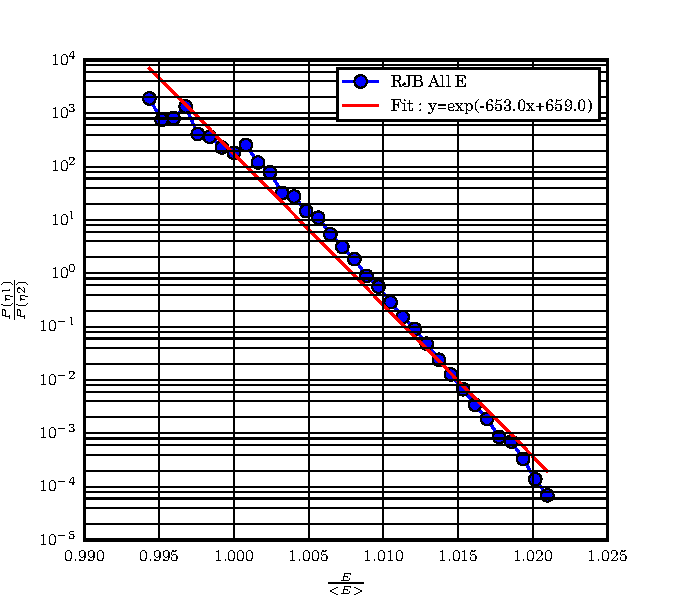
\includegraphics[width=1.0\textwidth]{{Figures/sumsq/RJBSumSqHistLogR6L144-alph1-476}.pdf}
	  \captionof{figure}{Total energy probability ratio for \rjb. }
  \label{fig:rjbsumsq}
\end{minipage}
}%
\caption{Total energy probability ratio for the \ofc\ and \rjb\ models for $\alpha=0.0476$, $L=144$, and $R=6$. Resulting fits are in agreement.}
\end{figure}%%
%%
The value of this proposed energy is that it closes the gap in the \ofc\ model relative to the \rjb\ model by the availability of a well defined energy.

% add subsection title
% group subsection by collected ideas in a more clear way
\subsection{Effectivity ergodicity in the \lr\ \ofc\ model}

To further establish the equilibrium behavior the work of Thirumalai and Mountain~\cite{thirm89} on ergodicity was used to establish the effective ergodic behavior of this system. Following Thirumalai-Mountain this metric can be used to determine effective ergodicity. The Thirumalai-Mountain metric in Eqn.~\eqref{eq:tmmetric} compares the time average stress ${<}\sigma{>}_t$ with the ensemble average$ {<}\sigma{>}_N$. %%
%%
\begin{figure}[!h]
    \centering
\makebox[\textwidth][c]{
      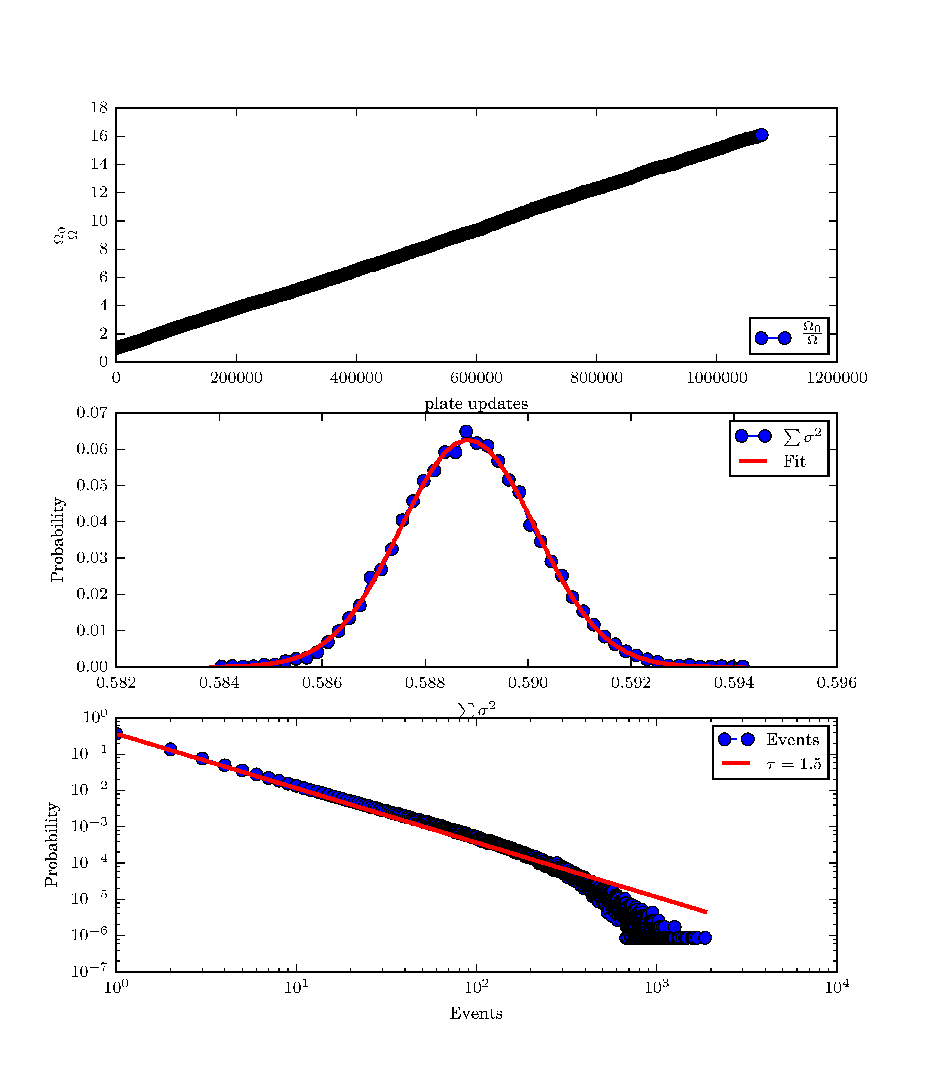
\includegraphics[scale=1.0]{{Figures/sumsq/SumSqHist4L120-alph1-0.05-noise-0.22}.pdf}
}
    \caption{Thirumalai-Mountain metric/energy/event size probability for the \ofc\ model with $\eta=0.22$, $\alpha=0.05$, $L=120$, and $R=4$. Equilibrium behavior is observed in all three measures.
    } 
  \label{fig:ofcmetricsumsq}
\end{figure}%%
%%
%%
%%
\begin{equation}
	\label{eq:tmmetric}
	\Omega = \frac{1}{N} \sum_i^N (<\sigma>_t-<\sigma>_N)^2 
\end{equation} %%
%%
For an effectively ergodic system the Thirumalai-Mountain metric must satisfy the following relation:  %%
%%
\begin{equation}
	\label{eq:tm_t}
 \frac{1}{\Omega}  \propto  t.
\end{equation} %%
%%
Figure~\ref{fig:ofcmetricsumsq} shows the equilibrium behavior of an \ofc\ system with parameters ($\eta=0.22$, $\alpha=0.05$, $L=120$, and $R=4$) by measuring  the Thirumalai-Mountain metric, the proposed energy, and event size probability distribution. The figure displays the agreement of all the equilibrium indicators for a system with \lr\ stress transfer and a fair amount of noise in the residual stress.